% Chapter Template

\chapter{Ensayos y resultados} % Main chapter title

\label{Chapter4} % Change X to a consecutive number; for referencing this chapter elsewhere, use \ref{ChapterX}
En este capítulo se explica cómo fueron los ensayos que se realizaron sobre el sistema y qué resultados se obtuvieron a partir de ellos.

%----------------------------------------------------------------------------------------
%	SECTION 1
%----------------------------------------------------------------------------------------
\section{Ensayos sobre la aplicación}
\label{sec:pruebasAPP}

En esta etapa se realizaron ensayos sobre la aplicación móvil de forma independiente, con el objetivo de validar su funcionamiento antes de su integración con el sistema embebido.

Para ello, se utilizó el entorno de desarrollo provisto por Ionic mediante el comando \texttt{ionic serve}, que permite ejecutar la aplicación en un navegador web. Este entorno facilitó el acceso a herramientas de depuración, tales como la simulación de distintos tamaños de pantalla y la visualización de mensajes en la consola.

La figura \ref{fig:ionic_debug} muestra el entorno de ejecución utilizado durante los ensayos.

\begin{figure}[h]
	\centering
	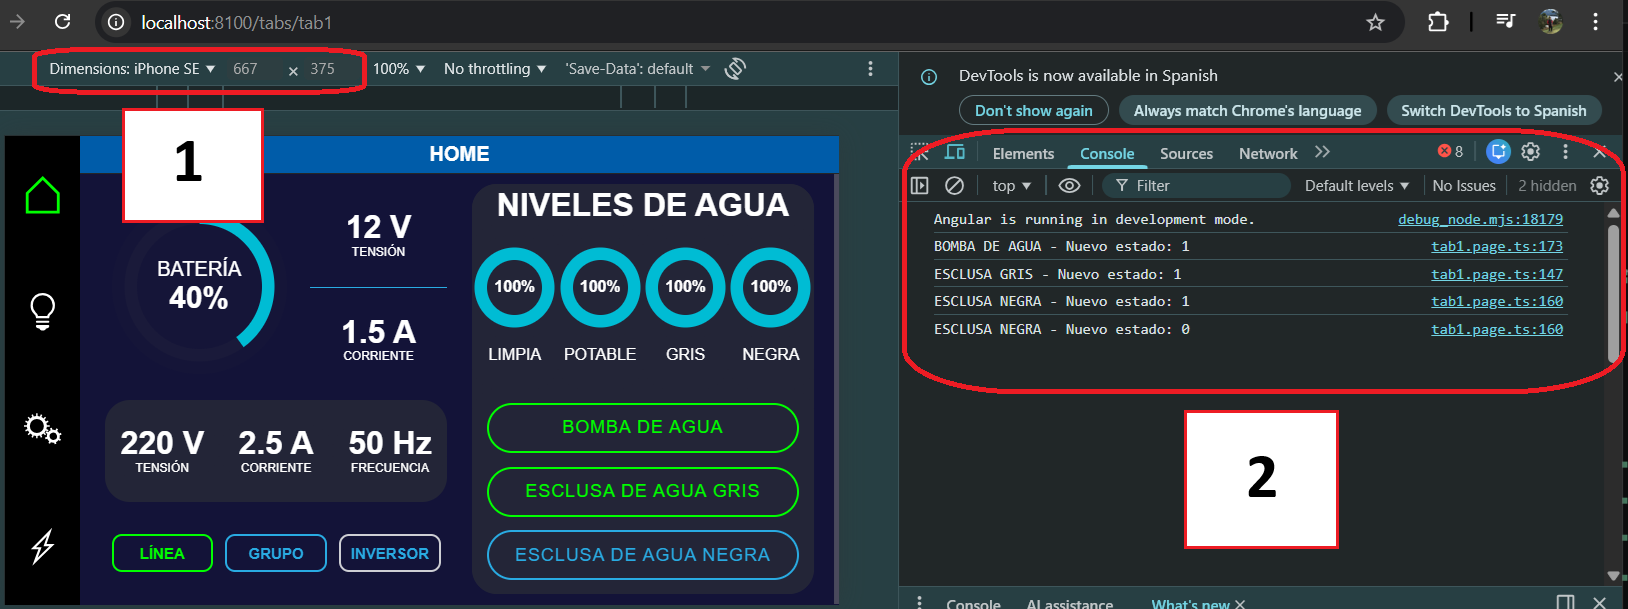
\includegraphics[scale=0.32]{./Figures/ionic_debug.png}
	\caption{Entorno de ejecución y depuración de la aplicación.}
	\label{fig:ionic_debug}
\end{figure}

En el sector identificado como cuadro 1, se empleó la funcionalidad de simulación de distintos tamaños de pantalla, lo que permitió evaluar el comportamiento de la interfaz frente a diferentes resoluciones.
\newpage
Por otro lado, en el cuadro 2 se encuentra la consola del navegador, donde se visualizaron mensajes de depuración generados mediante instrucciones como \texttt{console.log()}. Estos mensajes incluyeron valores de variables y estructuras de datos en formato \texttt{JSON}, lo que facilitó el seguimiento del estado interno de la aplicación y la detección de errores durante su ejecución.

El procedimiento de ensayo consistió en navegar entre las distintas pestañas de la aplicación, accionar los controles disponibles y observar el comportamiento de la interfaz. En paralelo, se analizaron los mensajes generados en la consola del navegador mediante instrucciones de depuración incorporadas en el código.

Adicionalmente, se implementó un esquema de prueba basado en la modificación manual de variables internas (\textit{hardcodeo}), con el fin de simular distintos estados del sistema. Esto permitió evaluar la forma en que la aplicación representa en pantalla valores correspondientes a diferentes condiciones de operación.

Como resultado, se verificó que la navegación entre pantallas se realizaba correctamente, que los controles respondían a las acciones del usuario y que los indicadores visuales reflejaban de manera coherente los valores asignados durante las pruebas.

Asimismo, se comprobó que la interfaz mantenía un comportamiento consistente frente a distintos tamaños de pantalla, sin presentar errores de visualización ni desajustes en la distribución de los elementos.

A partir de estos ensayos, se concluyó que la aplicación presentaba un funcionamiento adecuado a nivel de interfaz y lógica interna, lo que permitió avanzar hacia su integración con el sistema basado en ESP32.

\section{Ensayos sobre el sistema}
\label{sec:pruebasAPP_ESP32}

En esta etapa se realizaron ensayos de integración entre la aplicación móvil y el sistema basado en ESP32, con el objetivo de validar la comunicación entre ambos y el correcto funcionamiento del servidor implementado en el microcontrolador.

Para ello, se utilizó el entorno de ejecución de la aplicación en el navegador web, junto con el monitor serie del IDE Arduino, empleado para visualizar mensajes de depuración generados por el firmware del ESP32.

El montaje de ensayo consistió en conectar el ESP32 a una red Wi-Fi local, compartida con la computadora en la que se ejecutaba la aplicación. 

Al establecer la conexión, el microcontrolador informó su dirección IP a través del monitor serie, lo que permitió acceder a los endpoints del servidor desde la aplicación.

El procedimiento de prueba incluyó el acceso a los distintos endpoints mediante solicitudes HTTP de tipo GET, así como el envío de comandos a través de solicitudes POST generadas desde la interfaz.

Con el fin de evaluar la comunicación, se implementó en el firmware una función temporal que asignaba valores aleatorios a las variables contenidas en las estructuras \texttt{JSON}. Estos valores eran informados mediante mensajes en el monitor serie.

A partir de este esquema, se compararon los valores reportados por el ESP32 con los recibidos por la aplicación, y se verificó su coincidencia junto con su correcta representación en la interfaz.

La figura \ref{fig:app_json_recibido} muestra un ejemplo del archivo \texttt{JSON} recibido desde el endpoint home, que contiene tanto variables del sistema como estados de los pulsadores.

\begin{figure}[h]
	\centering
	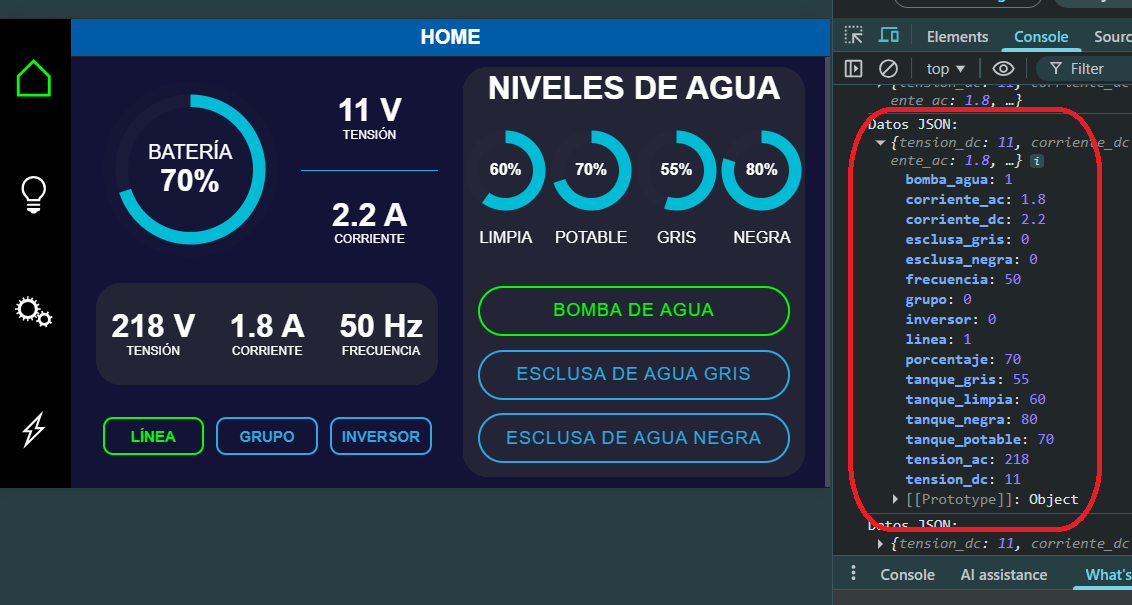
\includegraphics[scale=0.46]{./Figures/app_json_recibido.png}
	\caption{Archivo \texttt{JSON} recibido en la pestaña home.}
	\label{fig:app_json_recibido}
\end{figure}

Por otra parte, se evaluó el envío de comandos desde la aplicación hacia el ESP32 mediante solicitudes POST. La figura \ref{fig:pulsador_respuesta_esp32} muestra el mensaje recibido por el microcontrolador al accionar el pulsador correspondiente a la bomba de agua.

\begin{figure}[h]
	\centering
	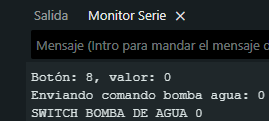
\includegraphics[scale=1]{./Figures/pulsador_respuesta_esp32.png}
	\caption{Mensaje recibido por el ESP32 al accionar un pulsador desde la aplicación.}
	\label{fig:pulsador_respuesta_esp32}
\end{figure}

En este caso, el identificador del comando y el valor asociado fueron correctamente interpretados por el sistema, lo que dio lugar al envío de la instrucción correspondiente hacia el módulo PRC10.

Asimismo, se verificó la respuesta del servidor ante estas solicitudes. La figura \ref{fig:app_json_pulsador} presenta el contenido de la respuesta enviada por el ESP32, donde se confirma el comando ejecutado junto con el nuevo estado asignado.

\begin{figure}[h]
	\centering
	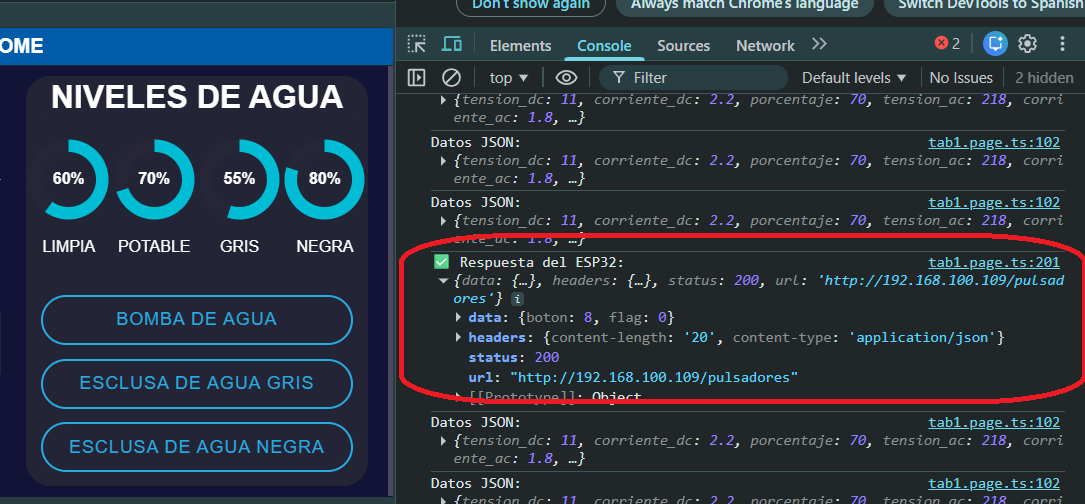
\includegraphics[scale=0.46]{./Figures/app_json_pulsador.png}
	\caption{Respuesta del servidor ante una solicitud de control.}
	\label{fig:app_json_pulsador}
\end{figure}

Como resultado, se comprobó que los datos intercambiados entre la aplicación y el ESP32 coincidían de manera consistente, que los comandos enviados eran correctamente procesados y que las respuestas del servidor reflejaban el estado actualizado del sistema.

A partir de estos ensayos, se concluyó que la comunicación entre la aplicación y el microcontrolador resultó confiable, lo que permitió validar el funcionamiento del servidor y avanzar hacia la etapa de pruebas con equipos reales.

\section{Ensayos de laboratorio}
\label{sec:ensayos_laboratorio}

En esta etapa se realizaron ensayos con equipos reales de la red de domótica de Enertik, con el objetivo de validar el funcionamiento del sistema en condiciones representativas de operación.

La figura \ref{fig:prc10} muestra el módulo PRC10 utilizado durante los ensayos. Este equipo fue separado y destinado específicamente a este desarrollo.

\begin{figure}[h]
	\centering
	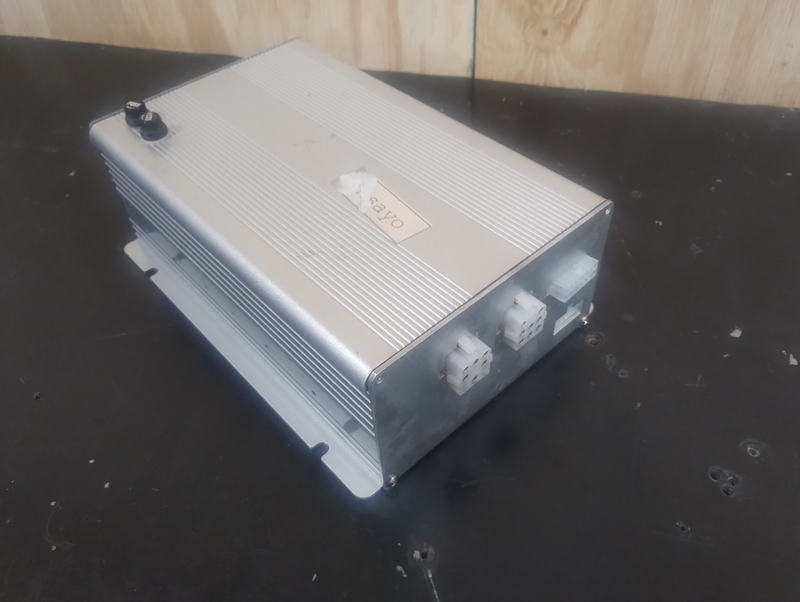
\includegraphics[scale=0.6]{./Figures/prc10.png}
	\caption{Módulo PRC10 utilizado en los ensayos.}
	\label{fig:prc10}
\end{figure}

Para la realización de las pruebas, se utilizó un maletín provisto por Enertik que integra los equipos comerciales empleados en aplicaciones de motorhomes. Este conjunto reproduce la configuración real del sistema, tanto a nivel de alimentación como de comunicación.

La figura \ref{fig:equipos_enertik} muestra dicho entorno, donde los dispositivos se encuentran interconectados mediante un cableado de cuatro conductores. En la misma se identifican el prototipo desarrollado (cuadro 1) y el módulo PRC10 (cuadro 2).

\begin{figure}[h]
	\centering
	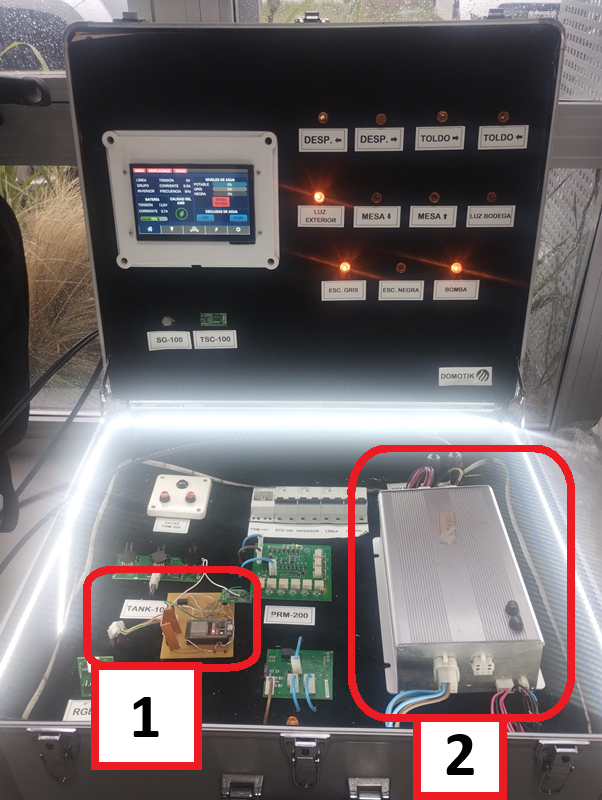
\includegraphics[scale=0.6]{./Figures/maletin.png}
	\caption{Equipos Enertik utilizados en los ensayos.}
	\label{fig:equipos_enertik}
\end{figure}

El sistema dispone de dos entradas de alimentación: una fuente de 12 V en corriente continua, que representa la batería, y una entrada de corriente alterna que simula las fuentes de línea, grupo electrógeno e inversor. Como carga, se utilizaron luces testigo que permiten visualizar el accionamiento de los distintos circuitos.

Para la integración con el ecosistema Victron, se emplearon un módulo Cerbo GX y un equipo MultiPlus-II 12/3000/120-32 230V \citep{web_multiplus}, tal como se muestra en la figura \ref{fig:equipos_victron}.

\begin{figure}[h]
	\centering
	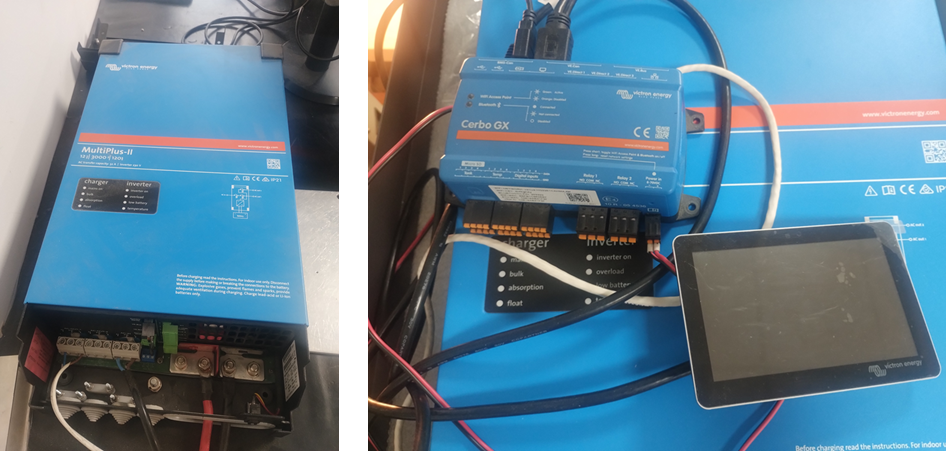
\includegraphics[scale=0.54]{./Figures/multiplus.png}
	\caption{Equipo Victron MultiPlus-II y módulo Cerbo GX.}
	\label{fig:equipos_victron}
\end{figure}

El procedimiento de ensayo consistió en instalar la aplicación en un dispositivo móvil con sistema operativo Android, establecer la conexión a la red Wi-Fi generada por el ESP32 y evaluar el comportamiento de cada una de las pestañas.

En la pestaña principal se accionaron los pulsadores y se verificó la respuesta de las luces testigo asociadas. Asimismo, se aplicaron variaciones sobre los sensores de nivel de los tanques, con el fin de simular distintos estados y comprobar la actualización de los indicadores en la interfaz.

Este procedimiento se replicó en las demás pestañas, donde se evaluaron los distintos controles implementados y su efecto sobre los dispositivos físicos del sistema.

En relación con la comunicación con los equipos Victron, se utilizó la pestaña energía para controlar el equipo MultiPlus. 

Al activar el Multiplus en modo inversor, el equipo comenzó a convertirla tensión
de batería en una señal alterna de 220 V. Como carga, se conectó un soldador de
tipo \textit{cautín} de alta potencia, lo que permitió observar la variación de la potencia
indicada en la aplicación.

Por otro lado, se conectó el Multiplus a la red domiciliaria y se lo configuró en
modo cargador. Mediante el uso de una pinza amperométrica, se verificó que el
valor de corriente de carga mostrado en la aplicación resultaba coherente con la
medición real.

Como criterio de validación, se consideró satisfactorio que los estados de los actuadores coincidieran con las acciones realizadas desde la aplicación, y que las variables medidas presentaran valores coherentes con las lecturas obtenidas mediante instrumentos externos.

Los resultados obtenidos indicaron que el sistema respondió correctamente a las acciones de control, tanto en los dispositivos de la red de Enertik como en los equipos del ecosistema Victron. Las magnitudes eléctricas visualizadas en la aplicación resultaron consistentes con las mediciones realizadas.

Adicionalmente, se realizó una prueba en un motorhome real durante una visita a la fábrica, donde se evaluaron los controles en condiciones reales de operación. En esta instancia, el sistema presentó un comportamiento adecuado y consistente con los ensayos de laboratorio.

No obstante, no fue posible validar la comunicación con equipos Victron en el vehículo, debido a la ausencia de este equipamiento en la unidad ensayada. Esta verificación queda planteada como trabajo futuro.

Finalmente, debido a restricciones de la empresa fabricante, no se dispuso de registros fotográficos de los ensayos realizados en el motorhome.